% Template for Cogsci submission with R Markdown

% Stuff changed from original Markdown PLOS Template
\documentclass[10pt, letterpaper]{article}

\usepackage{cogsci}
\usepackage{pslatex}
\usepackage{float}
\usepackage{caption}

% amsmath package, useful for mathematical formulas
\usepackage{amsmath}

% amssymb package, useful for mathematical symbols
\usepackage{amssymb}

% hyperref package, useful for hyperlinks
\usepackage{hyperref}

% graphicx package, useful for including eps and pdf graphics
% include graphics with the command \includegraphics
\usepackage{graphicx}

% Sweave(-like)
\usepackage{fancyvrb}
\DefineVerbatimEnvironment{Sinput}{Verbatim}{fontshape=sl}
\DefineVerbatimEnvironment{Soutput}{Verbatim}{}
\DefineVerbatimEnvironment{Scode}{Verbatim}{fontshape=sl}
\newenvironment{Schunk}{}{}
\DefineVerbatimEnvironment{Code}{Verbatim}{}
\DefineVerbatimEnvironment{CodeInput}{Verbatim}{fontshape=sl}
\DefineVerbatimEnvironment{CodeOutput}{Verbatim}{}
\newenvironment{CodeChunk}{}{}

% cite package, to clean up citations in the main text. Do not remove.
\usepackage{cite}

\usepackage{color}

% Use doublespacing - comment out for single spacing
%\usepackage{setspace}
%\doublespacing


% % Text layout
% \topmargin 0.0cm
% \oddsidemargin 0.5cm
% \evensidemargin 0.5cm
% \textwidth 16cm
% \textheight 21cm

\title{``I won't lie to you, your talk wasn't amazing'': Modeling polite
(in)direct remarks}


\author{{\large \bf Erica J. Yoon}, {\large \bf Michael Henry Tessler}, {\large \bf Noah D. Goodman} \and {\large \bf Michael C. Frank}  \\
        \{ejyoon, mtessler, ngoodman, mcfrank\} @stanford.edu \\ 
        Department of Psychology, Stanford University}

\begin{document}

\maketitle

\begin{abstract}
Why do people speak politely? Previous work has suggested that people
expect others to speak based on their desires to be transfer accurate
information (epistemic goal) and to make the listener feel good (social
goal), sometimes causing them to produce white lies (Yoon, Tessler,
Goodman, \& Frank, 2016). In the current work, we expand on this theory
to consider another prominent case of polite speech: indirect remarks.
We show that people expect a speaker to produce more of vague indirect
remarks (e.g. ``It wasn't amazing'') when there is greater risk of face
threat and the speaker wants to be considerate and informative at the
same time. We also compare goal attributions to speakers who produce
direct versus indirect remarks, and find that, when face threat risks
are high, people attribute more extreme tradeoff decisions between the
epistemic vs.~social goal for direct remarks, but report greater balance
between the two goals for indirect remarks. FIXME: These results align
with our model predictions, demonstrating great generalizability of our
model.

\textbf{Keywords:}
Politeness; computational modeling; communicative goals; pragmatics
\end{abstract}

\section{Introduction}\label{introduction}

Language users hear and produce \emph{polite speech} on a daily basis.
But being polite conflicts with one important goal of cooperative
communication: exchanging information efficiently and accurately (Grice,
1975). To be polite, people produce indirect requests that are much
longer than simple imperatives (``It would be great if you could close
that window'' as opposed to ``Close that window.''), and tell white lies
to make others feel good (``Your new dress is gorgeous!'') Thus,
speakers convey information inefficiently and risk losing accurate
information (indirect remarks) or even intentionally convey wrong
information (lies). If information transfer was the only currency in
communication, a cooperative speaker would find polite utterances
undesirable because they are potentially misleading.

However, people do speak politely. Adults and even young children
spontaneously produce requests in polite forms (Axia \& Baroni, 1985;
Clark \& Schunk, 1980), and speakers use politeness strategies even
while arguing, preventing unnecessary offense to their interactants
(Holtgraves, 1997).

Do these facts about politeness imply that people are not cooperative
communicators in the Gricean sense? Brown \& Levinson (1987) recast the
notion of a \emph{cooperative speaker} as one who has both an epistemic
goal to improve the listener's knowledge state as well as a social goal
to minimize any potential damage to the hearer's (and the speaker's own)
self-image, which they called \emph{face}. In their analysis, if the
speaker's intended meaning contains no threat to the speaker or
listener's face, then the speaker will choose to convey the meaning in
an efficient manner, putting it \emph{on the record}. As the degree of
face-threat becomes more severe, however, a speaker will choose to be
polite by producing more indirect utterances.

Based on Brown \& Levinson (1987), in our previous work, we argued that
language users think about polite speech as reflecting a tradeoff
between information transfer and face-saving (Yoon et al., 2016). When a
speaker tries to save face, she hides or risks losing information in her
intended message by making her utterance false or indirect to some
degree. On the other hand, when a speaker prioritizes truthfulness and
informativity, she may risk losing the listener's (or the speaker's own)
face. We developed a novel computational model that captures the idea
that cooperative speakers attempt to balance between the two goals:
information transfer and face-saving. This model built on a recent
formal framework for modeling pragmatic language understanding, the
``rational speech act'' (RSA) model (M. C. Frank \& Goodman, 2012;
Goodman \& Stuhlmüller, 2013). We examined one specific phenomenon of
polite speech, white lies (e.g.~saying someone's performance was
``okay'' when in fact it was terrible), and predictions from our model
were confirmed by empirical data on people's inferences about the
relation between a speaker's goals (e.g.~to be nice vs.~honest),
utterances (``It was okay'') and the true states of the world
(objectively how good was the addressee's piano recital performance).

In this work, we expand on our previous work and examine another case
study of polite speech phenomena: indirect remarks. Through indirect
remarks, speakers try to convey a particular message in a more nuanced
way. This is different from white lies, in that speaker's intentions are
no longer hidden, but revealed with suboptimal efficiency.

Why would people speak indirectly? For example, why would it be better
to say ``I would love another glass of wine, thanks.'' than ``Pour me
more wine''? The latter more clearly conveys the guest's intention for
the waiter to pour more wine. But the former is less imposing on the
waiter, and circumvents an impression that the speaker is in a position
to give orders to the listener. Indeed, even when the implied meaning of
the requests is the same, people prefer requests whose literal meanings
ask for the listener's permission (``Could I ask you where Jordan Hall
is?'') to those with literal meanings that assume listener's obligation
to respond (``Shouldn't you tell me where Jordan Hall is?'') (Clark \&
Schunk, 1980). Indirect requests are complicated to manipulate for many
reasons, for example due to various possible semantic forms of
imperatives, and our proposed work focuses on \emph{indirect remarks} as
a simpler case study to begin with.

Indirect remarks may be used to reflect speaker's attempt to balance
between two goals assumed by our model: informativity and face-saving.
For example, if Ann hesitantly comments on a colleague's past
presentation by saying ``The presentation \emph{wasn't
amazing}\ldots{}'' she does not preclude the possibility that the
presentation was bad, so the utterance is now not a downright lie; and
Ann still tries to save Bob's face by not explicitly saying that it was
bad. Thus we hypothesize that, similar to white lies, indirect speech
reflects speaker's desires to balance between the goal to be informative
(convey information in the most direct manner possible) and the goal to
save the listener's face (make the listener feel good, or at least avoid
making them feel bad).

\section{Computational Model}\label{computational-model}

In the current work, we build on our previous formal model that assumes
speaker to choose utterances approximately optimally given a utility
function, a standard assumption made in family of RSA models (Goodman \&
Stuhlmüller, 2013; Yoon et al., 2016). We proposed that there are two
utilities considered by the speaker. First, \emph{epistemic utility}
refers to the amount of information a \emph{literal listener} would
still not know about world state \(s\) after hearing a speaker's
utterance \(w\) (\emph{surprisal} that the speaker would want to
minimize): \[U_{epistemic}(w; s) = \ln(P_{L_0}(s \mid w))\], and the
literal listener is a simple Bayesian agent that takes the utterance to
be true:

\[
P_{L_0}(s \mid w)\propto {w}(s) \cdot P(s)
\]

Second, \emph{social utility} is the expected utility of the state the
listener would infer given the utterance \(w\), which is related to the
intrinsic value of the state from the listener's viewpoint :

\[
U_{social}(w; s) = \mathbb{E}_{P_{L_0}(s \mid w)}[V(s)],
\] where \(V\) is a value function that maps states to subjective
utility values and thus captures the affective consequences for the
listener of being in state \(s\).

We defined the overall speaker utility to be a weighted combination of
epistemic and social utilities:

\[
U(w;s;  \hat{\beta}) = \beta_{epistemic}\cdot U_{epistemic} + \beta_{social} \cdot U_{social}.
\]

The speaker chooses utterances \(w\) softmax-optimally given the state
\(s\) and his goal weights \(\hat{\beta}\): \[
P_{S_1}(w \mid s, \hat{\beta}) \propto \mathrm{exp}(\lambda \cdot \mathbb{E}[U(w; s;  \hat{\beta})])\]

The pragmatic listener, denoted \(L_1\), infers the world state based on
this speaker model. We will assume the listener does not know exactly
how the speaker weights his competing goals, however. We assume the
pragmatic listener jointly infers the state \(s\) and the utility
weights of the speaker, \(\beta_{epistemic}\) and \(\beta_{social}\)
(Goodman \& Lassiter, 2015; Kao, Wu, Bergen, \& Goodman, 2014):

\[
P_{L_1}(s,  \hat{\beta} \mid w)\propto P_{S_1}(w \mid s,  \hat{\beta})\cdot P(s) \cdot P( \hat{\beta}) \]

Within our experimental domain, we assume there are five possible states
of the world corresponding to the value placed on a particular referent
(e.g.~rating deserved by the presentation the speaker is commenting on):
\(S = \{s_{1}, ..., s_{5}\}\). We further assume a uniform prior
distribution over possible states of the world. The states have
subjective numerical values \(V(s_{i}) = \alpha \cdot i\), where
\(\alpha\) is a scaling parameter (later inferred from data).

The current work builds on our previous formal model by adding simple
but key components to predict indirect remark production and
comprehension. First, there had previously been five possible
utterances: \{It was \emph{terrible}, \emph{bad}, \emph{okay},
\emph{good}, and \emph{amazing}\}, all direct assertions of specific
states (e.g. ``It was amazing'' would be true for the state of 5 but
untrue for the states of 1 or 2). To probe people's inferences about
indirect remarks, we added five utterances to the set: \{It
\emph{wasn't} terrible, bad, okay, good, and amazing\}. These utterances
indirectly address the referent by negating certain state. Second, the
cost of longer utterances (it is more costly to say ``It wasn't
terrible'' than ``It was amazing'' due to inclusion of negation; Goodman
\& Lassiter (2015)) was accounted for by assigning greater cost to
indirect remarks with negation (cost = 2) than direct remarks with no
negation (cost = 1), which affected the likelihood of production of
utterances \emph{a priori}. We implemented this model using the
probabilisitic programming language WebPPL (Goodman \& Stuhlmüller,
2014) and a complete implementation can be found at \url{FIXME}.

To confirm the predictions of our new model, we first measure the
literal semantics in Experiment 1, then use these to predict people's
responses in two subsequent experiments. In Experiment 2, we examine
people's expectations for speaker production of utterances \(u\) given a
state and a speaker's goal. In Experiment 3, we investigate listeners'
inferences about speakers' goals given an utterance and a state. Then we
compare the behavioral results to our model predictions, that people's
inferences are based on a model of a speaker with two utilities:
epistemic and social.

\section{Experiment 1: Literal
semantics}\label{experiment-1-literal-semantics}

Experiment 1 probed judgments of literal meanings of the target words
assumed by our model and used in all our experiments. These judgments
will be used as the expected literal meanings in our model.

\begin{CodeChunk}
\captionsetup{width=0.8\columnwidth}\begin{figure}[t]

{\centering 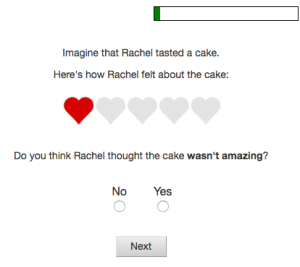
\includegraphics{figs/expt1_screen-1} 

}

\caption[Example of a trial in Experiment 1]{Example of a trial in Experiment 1.}\label{fig:expt1_screen}
\end{figure}
\end{CodeChunk}

\subsection{Method}\label{method}

\subsubsection{Participants}\label{participants}

25 participants with IP addresses in the United States were recruited on
Amazon's Mechanical Turk.

\subsubsection{Stimuli and Design}\label{stimuli-and-design}

We used 13 different context items that were previously used in Yoon et
al. (2016), in which someone evaluated a performance of some kind
(e.g.~presentation). For example, in one of the contexts, Bob saw a
presentation, and Bob's feelings toward Ann's cake (\emph{true state})
were shown on a scale out of five hearts (e.g.~two out of five hearts
filled in red color). The question of interest was ``Do you think Bob
thought the presentation was / wasn't X?'' where X could be one of five
possible words: \emph{terrible}, \emph{bad}, \emph{okay}, \emph{good},
and \emph{amazing}, giving rise to ten different possible utterances
(with negation or no negation). Each participant read 50 scenarios,
depicting every possible combination of 5 true states and 10 utterances.
The order of context items was randomized, and there were a maximum of
four repeats of each context item per participant.

\subsubsection{Procedure}\label{procedure}

Participants read scenarios and indicated their answer to each question
by answering ``No'' or ``Yes'' (see Figure 1 for a screenshot of an
example trial). The experiment can be viewed at:
\url{https://langcog.stanford.edu/expts/EJY/polgrice/negimp_prior_v1/negimp_prior.html}.

\begin{CodeChunk}
\captionsetup{width=0.8\textwidth}\begin{figure*}[b]

{\centering 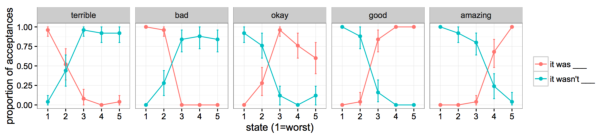
\includegraphics{figs/expt1_results-1} 

}

\caption[Results from Experiment 1]{Results from Experiment 1.}\label{fig:expt1_results}
\end{figure*}
\end{CodeChunk}

\subsubsection{Results}\label{results}

For this and all subsequent experiments, we analyze the data by
collapsing across context items. Meanings of the words as judged by
participants were as one would expect (see Figure 2). For utterances
without negation (e.g. ``It was terrible''), proportion of acceptances
for a word given the true state peaked where the degree of positivity,
neutrality and negativity of the state matched that of the word,
replicating literal semantics reported in Yoon et al. (2016). For
utterances with negation (e.g. ``It wasn't terrible''), proportion of
acceptances were inverses of acceptances for non-negated words. The
fraction of participants that endorsed utterance \(w\) for state \(s\)
will be used as the literal meaning \({w}(s)\) in Eq. 1.

\section{Experiment 2: Speaker
production}\label{experiment-2-speaker-production}

In Experiment 2, we examined people's predictions for the most likely
utterance produced by the speaker (\(u\)), given a description of the
true state of the world (e.g.~the speaker felt that a poem deserved 2
out of 5 hearts) and the speaker's goals (e.g.~the speaker wanted to
make the listener feel good). Critically, the contexts indicated face
threats toward the listener, as the speaker's utterance was an
evaluation of the listener's performance. We hypothesized that the
tradeoff in the speaker's intention to be informative versus to save the
listener's face would lead to greater use of vague, indirect remarks,
especially when the performance was poor.

\subsection{Method}\label{method-1}

\subsubsection{Participants}\label{participants-1}

202 participants with IP addresses in the United States were recruited
on Amazon's Mechanical Turk.

\subsubsection{Stimuli and Design}\label{stimuli-and-design-1}

We designed scenarios in which a person (e.g.~Ann) gave some performance
and asked for another person (e.g.~Bob)'s opinion on the performance.
The same context items and true states as Experiment 1 were used.
Additionally, we provided information on the speaker Bob's goal
(\emph{to make Ann feel good}, or \emph{to give as accurate and
informative feedback as possible}, or both) and the true state, or how
Bob actually felt Ann's performance (e.g.~2 out of 5 hearts), Then we
asked participants to predict what Bob would say, out of 10 possible
utterances (``It was terrible'', ``It was bad'' \ldots{} ``It wasn't
good'', ``It wasn't amazing''). Each participant read 15 scenarios,
depicting every possible combination of 3 goals and 5 states. The order
of context items was randomized, and there were a maximum of two repeats
of each context item per participant.

\subsubsection{Procedure}\label{procedure-1}

Participants read each scenario followed by a question that read, ``If
Bob wanted \emph{to make Ann feel good} (or \emph{to give accurate and
informative feedback}, or \emph{BOTH make Sarah feel good AND give
accurate and informative feedback}), what would Bob be most likely to
say?'' Participants indicated their answer by choosing one of the
options on the two dropdown menus, side-by-side, one for choosing
between \emph{was} vs. \emph{wasn't} and the other for choosing among
\emph{terrible}, \emph{bad}, \emph{okay}, \emph{good}, and
\emph{amazing} (see Figure 3). The experiment can be viewed at:
\url{https://langcog.stanford.edu/expts/EJY/polgrice/speaker_production_dropdown_v2/speaker.html}.

\subsection{Behavioral results}\label{behavioral-results}

\begin{CodeChunk}
\captionsetup{width=0.8\textwidth}\begin{figure}[b]

{\centering 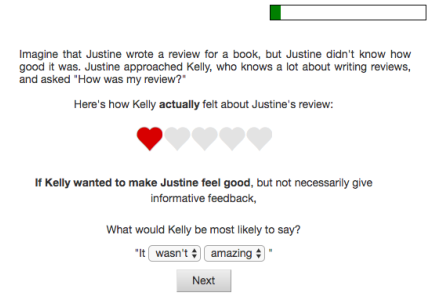
\includegraphics{figs/expt2_screen-1} 

}

\caption[Example of a trial in Experiment 2]{Example of a trial in Experiment 2.}\label{fig:expt2_screen}
\end{figure}
\end{CodeChunk}

People's predictions for speaker's utterances given varied depending on
speaker's goals, and these differences wre especially pronounced for
worse true states (Figure 4). For good states (4 and 5 hearts), positive
direct remarks were judged to be the most likely utterances across all
three goal conditions. For less-than-perfect, but still decent states,
there was a greater degree of expectation of white lies (e.g. ``It was
amazing'' for 4 hearts) given social goal. Our hypotheses were borne out
for bad states (1 and 2 hearts): there were more instances of expected
indirect remarks overall across all goal conditions given bad states.
Critically, speakers with both goals to be informative and socially
considerate were predicted to produce more indirect than direct remarks,
unlike the other two goal conditions (Figure 5). Thus, these results
indicated that a speaker who considers both informative and social
goals, and thus is in want of a compromise between the two, is expected
to produce relatively more indirect remarks.

\begin{CodeChunk}
\captionsetup{width=0.8\textwidth}\begin{figure*}[b]

{\centering 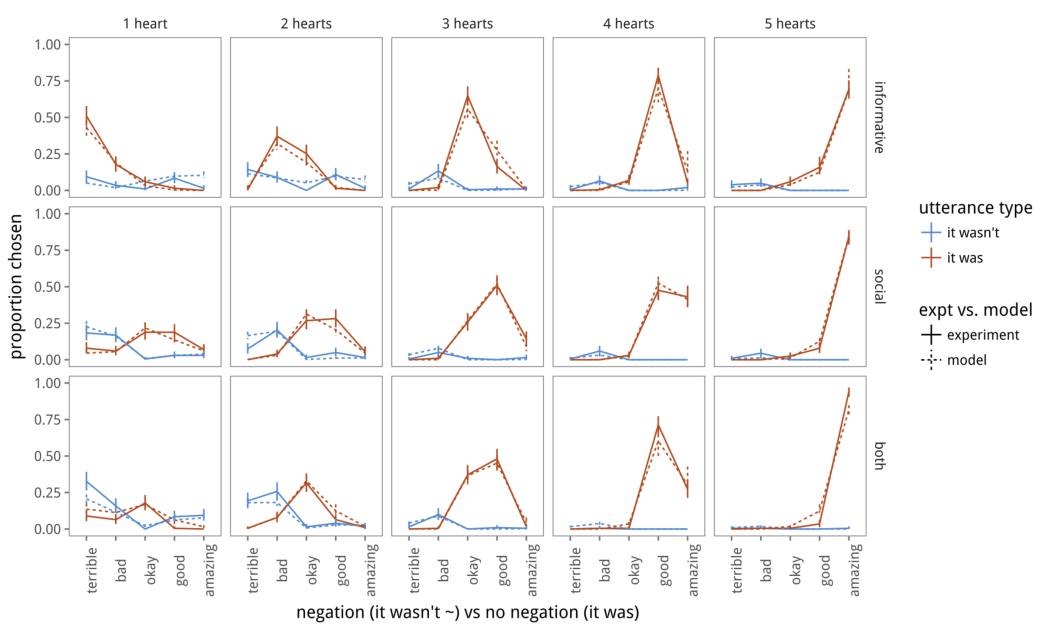
\includegraphics{figs/expt2_results-1} 

}

\caption[Results from Experiment 2]{Results from Experiment 2.}\label{fig:expt2_results}
\end{figure*}
\end{CodeChunk}

\begin{CodeChunk}
\captionsetup{width=0.8\textwidth}\begin{figure}[t]

{\centering 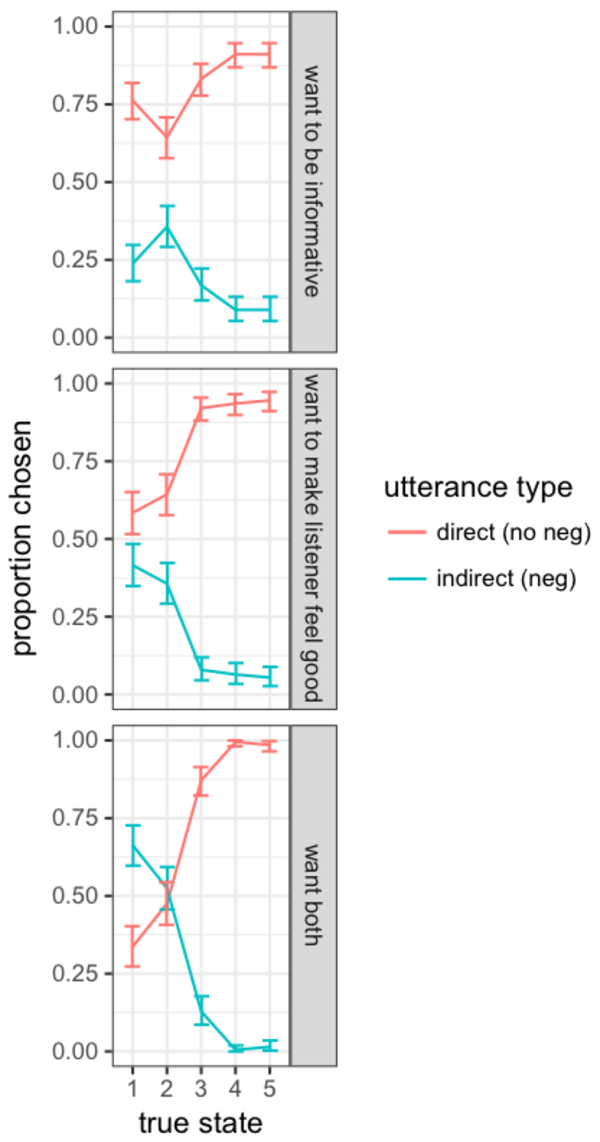
\includegraphics{figs/expt2_results2-1} 

}

\caption[Results from Experiment 2]{Results from Experiment 2.}\label{fig:expt2_results2}
\end{figure}
\end{CodeChunk}

\subsection{Model predictions}\label{model-predictions}

\subsubsection{Model fitting}\label{model-fitting}

\subsubsection{Results}\label{results-1}

\section{Experiment 3: Goal
inference}\label{experiment-3-goal-inference}

\subsection{Method}\label{method-2}

\subsubsection{Participants}\label{participants-2}

60 participants with IP addresses in the United States were recruited on
Amazon's Mechanical Turk.

\subsubsection{Stimuli and Design}\label{stimuli-and-design-2}

We presented the same context items and true states (i.e.~how Bob
actually felt towards Ann's performance) as Experiment 2, but instead of
goals we provided Bob's utterances (``It wasn't amazing''). Then we
asked participants to infer the likelihood of Bob's goals to \emph{to
make Ann feel good}, or \emph{to give accurate and informative
feedback}. Each participant was randomly assigned to one of two
conditions to read 25 scenarios, depicting half (counterbalanced) of all
possible combinations of 5 true states and 10 utterances. The order of
context items was randomized, and there were a maximum of two repeats of
each context item per participant.

\subsubsection{Procedure}\label{procedure-2}

Participants read each scenario followed by a question that read,
``Based on what Bob said, how likely do you think that Bob's goal was
to: \emph{to make Ann feel good}; \emph{to give accurate and informative
feedback}'' with the two goals placed in a random order next to two
slider bars, on which the participant could indicate each goal's
likelihood. The experiment can be viewed at:
\url{https://langcog.stanford.edu/expts/EJY/polgrice/L2_G_Neg/polgrice_L2_G.html}.

\subsection{Behavioral results}\label{behavioral-results-1}

\begin{CodeChunk}
\captionsetup{width=0.8\textwidth}\begin{figure*}[b]

{\centering 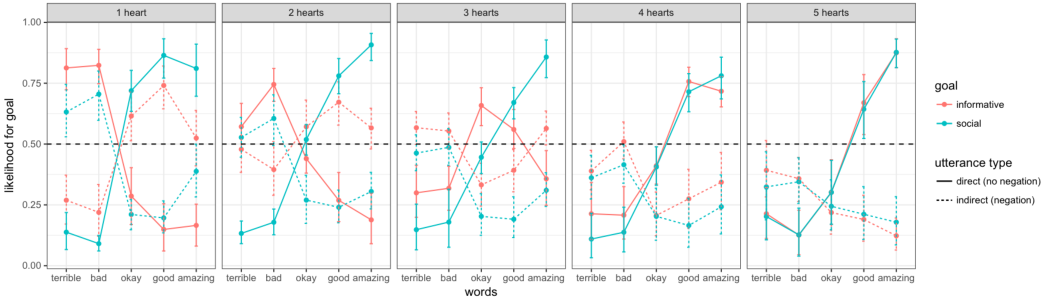
\includegraphics{figs/expt3_results-1} 

}

\caption[Results from Experiment 2]{Results from Experiment 2.}\label{fig:expt3_results}
\end{figure*}
\end{CodeChunk}

Participants rated speaker's goals differentially depending on the true
state and utterance (see Figure 6). Results for direct remarks with no
negation replicated our previous findings: Goal to be informative was
rated highest when the true state was most consistent with the literal
meanings. As direct remarks became more positive, participants increased
in their attribution of speaker's goal to make the listener feel good.

Comparison of direct versus indirect remarks revealed an interesting
asymmetry. For positive states (4 and 5 hearts), both informative and
social goal attributions increased with more positive valence of the
direct remarks, whereas both goal attributions mostly stayed low below
chance level across all indirect remarks. For negative states (1 and 2
hearts), interesting similarities and differences between the two types
of utterances were observed. Similarly between the two, there was a
crossover in goal attribution, caused by tradeoff between
utterance-meaning match (informative goal) and face-saving (social
goal). This tradeoff however is much more exaggerated in direct than
indirect remarks: saying ``It was amazing'' given a state of 1 heart
blatantly prioritizes social goal and forgos informative goal. On the
other hand, indirect remarks present a more balanced decision: saying
``It wasn't amazing'' moderately satisfies both goals. Again, this
finding confirms that a speaker who seeks a compromise between the goals
to be informative and to save face produces more indirect remarks, and
this desire then to be recognized by the listener.

\subsection{Model predictions}\label{model-predictions-1}

\subsubsection{Model fitting}\label{model-fitting-1}

\subsubsection{Results}\label{results-2}

\section{Discussion}\label{discussion}

In this work, we showed that our formal model with two speaker utilities
(epistemic and social) can be used to not only explain white lie
understanding but also indirect remark production and comprehension. As
we predicted, speakers were expected to produce more indirect remarks
when the listener's performance of concern was poorer, and thus the
listener's face was under threat, and when the speakers wanted a
compromise between the two conflicting goals (Experiment 2). Consistent
with this, participants inferred a greater balance of the two goals in
production of indirect remarks given bad true states.

An important contribution of this work is in showing the
generalizability of our formal model in two ways: extending to other
kinds of polite speech (white lies and indirect remarks), and predicting
comprehension as well as production of polite speech.

FIXME: some discussion about other approaches to indirect speech
(e.g.~Danescu-Niculescu-Mizil's work on polite requests)

\section{Acknowledgements}\label{acknowledgements}

\section{References}\label{references}

\setlength{\parindent}{-0.1in} \setlength{\leftskip}{0.125in} \noindent

\hypertarget{refs}{}
\hypertarget{ref-axia1985}{}
Axia, G., \& Baroni, M. R. (1985). Linguistic politeness at different
age levels. \emph{Child Development}, 918--927.

\hypertarget{ref-Brown1987}{}
Brown, P., \& Levinson, S. C. (1987). \emph{Politeness: Some universals
in language usage} (Vol. 4). Cambridge Univ. Press.

\hypertarget{ref-clark1980}{}
Clark, H. H., \& Schunk, D. H. (1980). Polite responses to polite
requests. \emph{Cognition}, \emph{8}(2), 111--143.

\hypertarget{ref-Frank2012}{}
Frank, M. C., \& Goodman, N. D. (2012). Predicting pragmatic reasoning
in language games. \emph{Science}, \emph{336}(6084), 998--998.

\hypertarget{ref-GoodmanLassiter2015}{}
Goodman, N. D., \& Lassiter, D. (2015). Probabilistic semantics and
pragmatics: Uncertainty in language and thought. In S. Lappin \& C. Fox
(Eds.), \emph{The handbook of contemporary semantic theory, 2nd
edition}. Wiley-Blackwell.

\hypertarget{ref-Goodman2013}{}
Goodman, N. D., \& Stuhlmüller, A. (2013). Knowledge and implicature:
Modeling language understanding as social cognition. \emph{Topics in
Cognitive Science}, \emph{5}.

\hypertarget{ref-dippl}{}
Goodman, N. D., \& Stuhlmüller, A. (2014). The Design and Implementation
of Probabilistic Programming Languages. \url{http://dippl.org}.

\hypertarget{ref-Grice1975}{}
Grice, H. P. (1975). Logic and conversation. In \emph{Readings in
language and mind}. Blackwell.

\hypertarget{ref-holtgraves1997}{}
Holtgraves, T. (1997). YES, but. positive politeness in conversation
arguments. \emph{Journal of Language and Social Psychology},
\emph{16}(2), 222--239.

\hypertarget{ref-Kao2014}{}
Kao, J. T., Wu, J. Y., Bergen, L., \& Goodman, N. D. (2014). Nonliteral
understanding of number words. \emph{Proceedings of the National Academy
of Sciences}, \emph{111}(33), 12002--12007.

\hypertarget{ref-yoon2016}{}
Yoon, E. J., Tessler, M. H., Goodman, N. D., \& Frank, M. C. (2016).
Talking with tact: Polite language as a balance between kindness and
informativity. In \emph{Proceedings of the thirty-eighth annual
conference of the Cognitive Science Society}.

\end{document}
